\documentclass{article}
%\documentclass[journal,12pt,twocolumn]{IEEEtran}
\usepackage{cite}
\usepackage{amsmath,amssymb,amsfonts,amsthm}
\usepackage{algorithmic}
\usepackage{graphicx}
\usepackage{textcomp}
\usepackage{tfrupee}
\usepackage{xcolor}
\usepackage{txfonts}
\usepackage{listings}
\usepackage{enumitem}
\usepackage{mathtools}
\usepackage{float}
\usepackage{gensymb}
\usepackage[breaklinks=true]{hyperref}
\usepackage{tkz-euclide} % loads  TikZ and tkz-base
\usepackage{listings}
\usepackage{gvv}
\title{Discrete}
\author{Hemant Katta}
\date{September 2023}

\begin{document}

\maketitle

%\section{SECTION A}
\begin{enumerate}
    \item If $-\frac{5}{7}$, $a$, $2$ are consecutive terms in an Arthimetic Progression, then the value of $a$ is 
    \begin{enumerate}
        \item $\frac{9}{7}$
         \item $\frac{9}{14}$
          \item $\frac{19}{7}$
           \item $\frac{19}{14}$
    \end{enumerate}
    \item If two positive integers $p$ and $q$ can be expressed as $p = ab^3$ and $q = a^2b$; 
$a$ and $b$ being prime numbers, then find LCM of ($p$, $q$) . 

    \item Show that any positive odd integer is of the form $4q + 1$ or $4q + 3$ for some integer $q$. 
    \item Prove that $\sqrt{5}$ is an irrational number.
    \item
    \begin{enumerate}
    \item Find the sum of first $16$ terms of an Arithmetic Progression whose $4^{\text{th}}$ and $9^{\text{th}}$ terms are $-15$ and $-30$ respectively.
    
        \item If the sum of first $14$ terms of an Arithmetic Progression is $1050$ and its fourth term is $40$, find its $20^{\text{th}}$ term.
    \end{enumerate}

    \item 
    \begin{enumerate}
        \item Find the sum of the first twelve $2$-digit numbers which are 
multiples of $6$.

        \item In an AP, if $a_2=26$ and $a _ {15} = -26$, then write the AP.
        \end{enumerate}
        \item In Mathematics, relations can be expressed in various ways. The 
matchstick patterns are based on linear relations. Different strategies 
can be used to calculate the number of matchsticks used in different 
		\figref{fig:ap} 
 \\One such pattern is shown below. Observe the pattern and answer the 
following questions using Arithmetic Progression :
\begin{figure}[H]
    \centering
	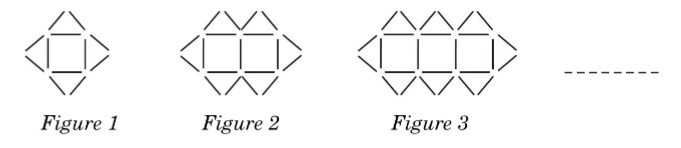
\includegraphics[width=\columnwidth]{figs/ap.jpg}
	\caption{patterns of Figure1, figure2 ,figure3}
    \label{fig:ap}
\end{figure}
    \begin{enumerate}
	    \item Write the AP for the number of triangles used in the \figref{fig:ap}. Also, 
write the nth term of this AP.
\item Which figure has $61$ matchsticks ? 
    \end{enumerate} 

    \item 
    \begin{enumerate}
        \item In an A.P. if the sum of third and seventh term is zero, find its $5^{\text{th}}$ term.
        
        \item Determine the AP whose third term is $5$ and seventh term is $9$.
        \end{enumerate}

    
        \item Find the sum of the first $20$ terms of an A.P. whose $n^{\text{th}}$ term is given as $a_n=5-2n$
    
    
        \item Find the common difference 'd' of an AP whose first term is $10$ and the sum of the first $14$ terms is $1505$.

        \item For what value of 'n', are the $n^{\text{th}}$ terms of the APs: $9,7,5,\dots$ and $15,12,9,\dots$ the same?

        \item
        \begin{enumerate}
            \item The curved surface area of a right circular cylinder is $176 sq.cm$ and its volume is $1232cu. cm$. What is the height of the cylinder?
            
        \item The largest sphere is carved out of a soild cube of side $21 cm$. Find the volume of the sphere.
        \end{enumerate}
        \item The sum of the first three terms of an A.P is $33$. If the product of first and third term exceeds the second term by $29$, find the A.P.
            
         \item
        \begin{enumerate}
            \item Find the number of terms in the following A.P:
            \begin{align}
                5,11,17,\dots,203
            \end{align}
 \item Find the sum of the first $20$ terms of an AP whose $n^{\text{th}}$ term is given as $a_n=5-3n$
        \end{enumerate}

        \item While buying an expensive item like a house or a car, it becomes easier for a middle-class person to take a loan from a bank and then repay the loan along with interest in easy instalments. 
          Aman buys a car by taking a loan of \rupee 2,36,000 from the bank and starts repaying the loan in monthly instalments. He pays \rupee 2,000 as the first instalment and then increases the instalment by \rupee 500 every month. 
        \begin{enumerate}
        \item Find the amount he pays in the $25^{\text{th}}$ installment.
\item Find the total amount paid by him in the first $25$ installments.
    \end{enumerate} 
       
        \end{enumerate}


\end{document}
